\documentclass[10pt, letterpaper]{article}
\usepackage[utf8]{inputenc}
\usepackage[spanish,es-nodecimaldot]{babel}
\usepackage[top=1in, bottom=1in, left=1in, right=1in]{geometry}
\usepackage{hyperref}
\usepackage{graphicx}
\graphicspath{{./assets/}}

\begin{document}

\begin{center}
    {\large \bfseries Modelado y Programación | Proyecto 1 \par}
    \vspace{0.2cm}
    Diego Jardón, Pablo Trinidad.
\end{center}

\section{Introducción}

A continuación se presentan los detalles del proyecto 1 del curso de Modelado y Programación
de la Facultad de Ciencias del semestre 2021-1 presentado por Diego Jardón y Pablo Trinidad.\\

Como fue descrito, el aeropuerto de la Ciudad de México tiene el requerimiento de obtener la
información del clima de vuelos que suceden a diario. Para esto nos fueron entregados dos datasets
(\texttt{dataset1.csv} y \texttt{dataset2.csv}) con información referente a algunos vuelos nacionales
e internacionales. El proyecto consta de un programa que utiliza dichos datasets para obtener la
información solicitada.\\

Se sugiere el uso de servicios web para obtener la información correspondiente del clima.

\section{Análisis del problema}

\subsection{Descripción}

Las locaciones estan dadas de dos formas distintas (nombre de ciudad y coordenadas geográficas).
Para cada locación se deberá regresar la información meteorológica correspondiente, que incluye (al menos)
temperatura (máximo y mínimo), sensación térmica y humedad.

La solicitud de datos meteorológicos se hará a través de \emph{datasets} de locaciones en cualquiera de los dos formatos (nombre de ciudad o coordenadas geográficas).

Dado que mostrar información acerca del clima de la Ciudad de México sería redudante pues el usuario ya cuenta con esa información, cuando la
locación de origen falte (dataset con nombre de ciudades), se asumirá que es la Ciudad de México y se obviará mostrar su información meteorológica.

\subsection{Requerimientos no funcionales}

\begin{enumerate}
  \item Se espera que las comunicación con el servicio web utilizado para obtener la información del
  clima pueda ser realizada de manera concurrente, es decir, debe tener la capacidad de realizar múltiples
  peticiones al servicio web de manera simultánea.
  \item El programa debe contar con un sistema básico de cache debe evitar realizar llamadas
  repetidas al servicio web y en su lugar utilizar las respuestas previamente obtenidas y
  almacenadas. 
\end{enumerate}

\section{Análisis y búsqueda de herramientas}
\subsection{Proveedores de información meteorológica}
El proveedor que seleccionamos fue \href{http://www.google.com}{OpenWeatherAPI} dado que se adaptaba a nuestras necesidades muy bien, pues soportaba búsqueda de datos meteorológicos por nombre de ciudad y por coordenadas, que era justo lo que necesitabamos.
\subsection{Sistema de cache}
La capa de caché fue implementada utilizando usando hash tables para evitar llamadas duplicadas. Siendo la llave la locación solicitada (nombre de la ciudad o código de aeropuerto) y los valores la respuesta de la API.
\subsection{Plataforma (lenguaje de programación)}
Decidimos utilizar el lenguaje programación Go pues nos facilitaría el manejo de las llamadas
concurrentes para lograr el punto extra :).

\section{Solución}
\subsection{Descripción general}

Se plantea una utilidad de línia de comandos que permita a los usuarios leer datasets en cualquiera
de los dos formatos previamente mencionados que exponga la siguiente interfáz:
\begin{center}
  \texttt{program -d DATASET -f FORMAT}
\end{center}
Donde \texttt{DATASET} es la ubicación (relativa o absoluta) del dataset en formato CSV y
\texttt{FORMAT} un valor entero en $\{1, 2\}$, donde 1 denota que el formato del dataset
es el de pares de aeropuertos con sus coordenadas y 2 un dataset donde la primera columna
contiene nombres de ciudades \footnote{Para más detalles por favor leer README.md}.

Puesto que el objetivo del programa es que sea reutilizable, se evita a toda costa incluir
en el código fuente (\textit{hardcoded}) particularidades como:
\begin{itemize}
  \item Ubicación de los datasets.
  \item Llaves (API keys) de los servicios utilizados.
\end{itemize}

El programa cumple con las limitantes y recomendaciones sobre el uso del API de OpenWeather a la
par que reduce el número de llamadas al mínimo indispensable. Las llamadas al API son realizadas
de manera concurrente de forma que no se tengo que esperar a que una concluya para poder realizar
las siguientes.

\subsection{Organización de los componentes}

Con el objetivo de cumplir con los principios \textbf{SOLID} se plantean tres grandes componentes
del programa:
\begin{enumerate}
  \item \textbf{La aplicación principal} (\texttt{cli/}), quien se encarga de inicializar el programa
  con los datos dados, i.e: API keys, leer y validar el formato de los datasets. Y también se
  encarga de mostrar información relevante al usuario respecto a la ejecución del programa así
  como los resultados meteorológicos obtenidos.
  \item \textbf{La capa de acceso a los datos} (\texttt{store/}), quien se encarga de proveer la
  información meteorológica a partir de las consultas recibidas. Esta es importante pues abstrae
  los detalles de acceso a los datos (cache y concurrencia) de la aplicación principal.
  \item \textbf{La comunicación con el API} (\texttt{store/openweather}), quien realiza la
  comunicación directa con los servicios de OpenWeather y expone métodos con dicho propósito.
\end{enumerate}

Es importante mencionar que la separación que se decidió realizar permite que aunque la forma
de leer los datasets o comunicar los resultados cambie, la capa de acceso a los datos es ajena
a dichos cambios puesto que no comparte responsabilidades directamente.

Así mismo, se siguió el principio de inversión de dependencias que permite que los módulos
dependan de abstracciones y \textit{contratos} pero no de implementaciones particulares.
Esto a su vez genera la posibilidad de probar módulos y sus dependencias sin necesariamente
llamar a los servicios (\textit{mocked implementations}).\\

\textbf{Nota importante}: Todo el código dentro de \texttt{store}, es decir, los paquetes de Go \\
\texttt{github.com/pablotrinidad/weatherreport/store} y\\
\texttt{github.com/pablotrinidad/weatherreport/store/openweather}
cumplen con 100\% de covertura en pruebas unitarias. Esto es importante porque nos permite probar
como se comportarán cuando se reciba información inesperada o sucedan casos extremos.

\subsection{Diagramas de flujo}
Sobre la ejecución general del programa:
\begin{center}
  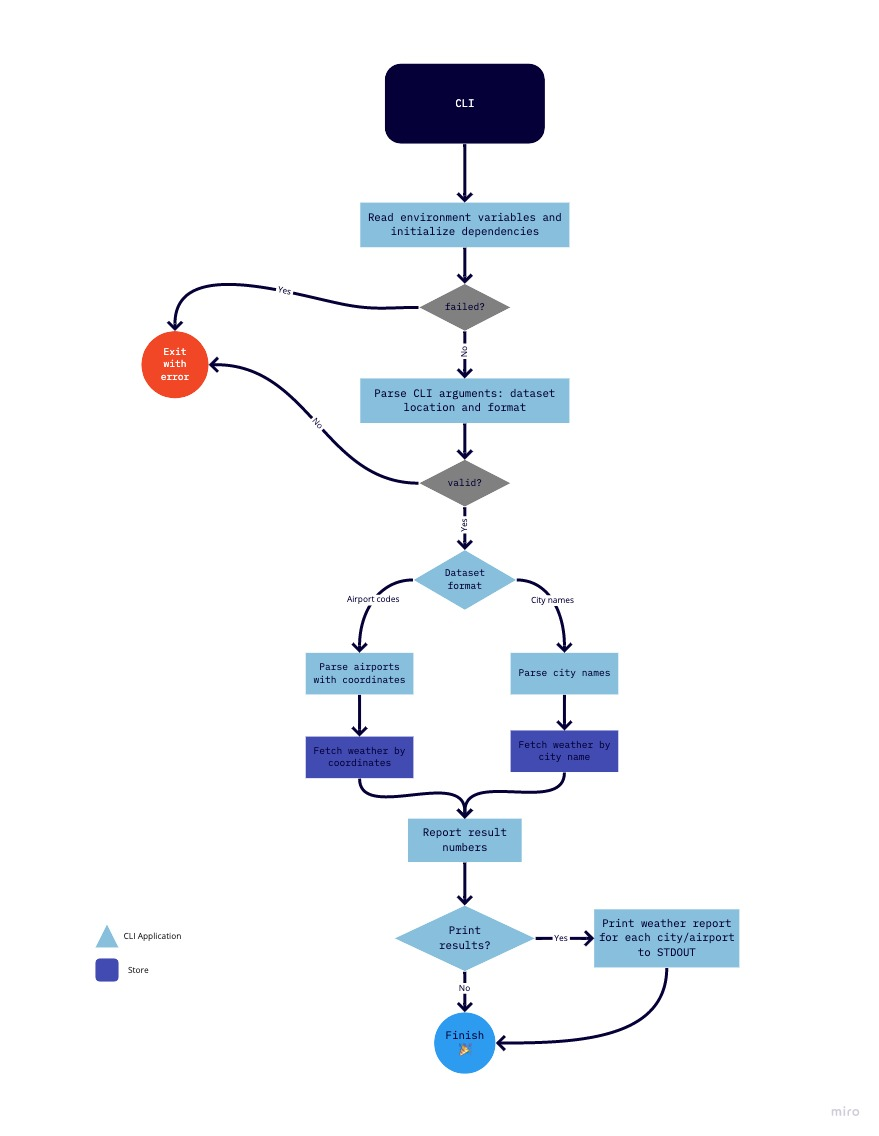
\includegraphics[scale=0.5]{flow-chart-1.jpg}
\end{center}
\clearpage
Implementación concurrente de interfaz \texttt{Store} dentro de\\
\texttt{github.com/pablotrinidad/weatherreport/store}:

\begin{center}
  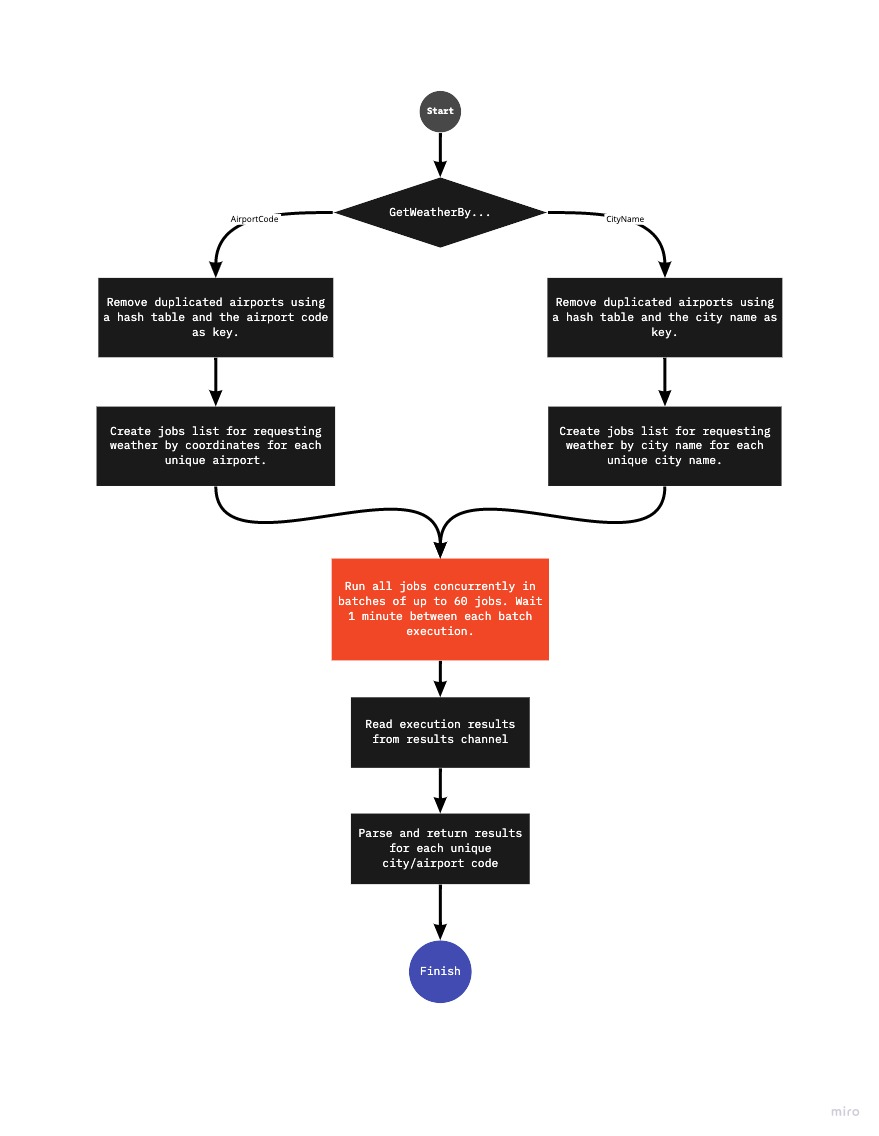
\includegraphics[scale=0.5]{flow-chart-2.jpg}
\end{center}
\clearpage

Detalles del manejo de ejecución concurrente de tareas por lotes\\
(\texttt{store/concurrentstore.go} $\rightarrow$ \texttt{fetchConcurrently(...)})
\begin{center}
  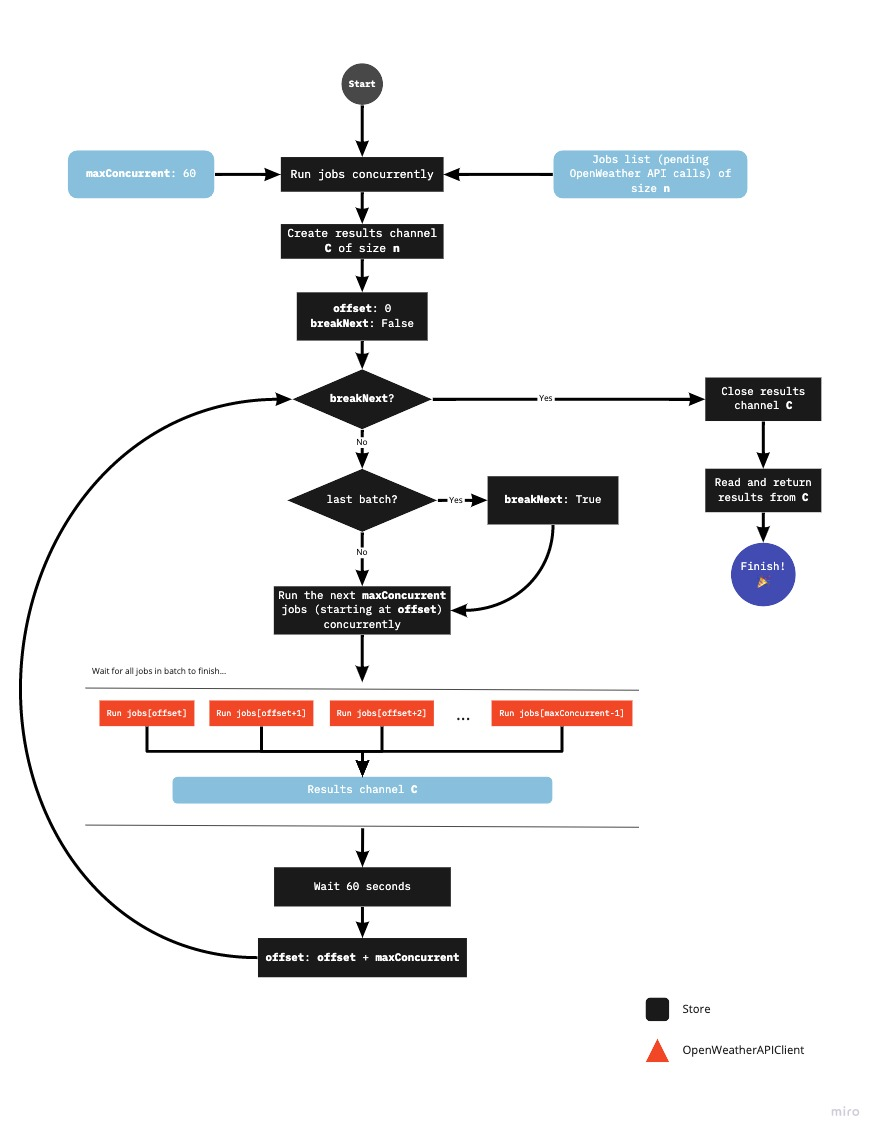
\includegraphics[scale=0.5]{flow-chart-3.jpg}
\end{center}
\clearpage

\subsection{Presupuesto}
En principio, manejaríamos el presupuesto en términos de horas, con un costo de 200.00 M.N. la hora de trabajo por persona. Dado que el equipo consiste de 2 personas el costo por hora del proyecto sería 400.00 M.N., se estimaron necesarias aproximadamente 30 horas para la realización del proyecto, lo que resulta en 12,000 M.N.

Nota: el presupuesto anterior contempla solamente el desarrollo inicial con 2 revisiones finales para corregir errores que afecten gravemente la funcionalidad prencipal. El mantenimiento y posteriores actualizaciones no están incluidas en el presupuesto. 
\section{Mejoras a futuro}
\begin{enumerate}
    \item Mejorar las pruebas a las llamadas concurrentes para no tener que esperar el minuto completo (mock clock) entre batches de peticiones.
    \item Dado que las aplicaciones de terminal (CLI) no suelen ser muy amigables para los usuarios. Probablemente haga sentido abandonar este formato de interfaz de usuario y trabajar una versión más amigable como en una GUI o proveer una salida estandarizada (CSV) con los resultados. 
    \item Darle soporte a más funcionalidad de OpenWeatherAPI, como buscar por codigo postal o por zona rectangular o circular, etcétera.
    \item Estandarizar los formatos de entrada y salida de forma que podamos evitar inconsitencias.
    \item Dar soporte a visualización del clima a través de un mapa con elementos dinámicos.
\end{enumerate}

\end{document}